\documentclass[aspectratio=169, 12pt]{beamer}
\usepackage[UTF8]{ctex}
\usepackage{graphicx}
\usepackage{booktabs}
\usepackage{listings}
\usepackage{xcolor}
\usepackage{tikz}
\usepackage{amsmath}
\usepackage{hyperref}

% --- 主题风格 ---
\usetheme{Madrid}
\usecolortheme{whale}
\usefonttheme{professionalfonts}

% --- 代码高亮设置 ---
\lstset{
    language=Python,
    basicstyle=\ttfamily\small,
    keywordstyle=\color{blue},
    commentstyle=\color{green!60!black},
    stringstyle=\color{orange},
    breaklines=true,
    frame=single,
    showstringspaces=false,
    backgroundcolor=\color{gray!5}
}

% --- 自定义命令 ---
\newcommand{\highlight}[1]{\textcolor{red}{\textbf{#1}}}

\title[CV导论与图像基础]{第1周:计算机视觉导论与图像基础}
\subtitle{让机器“看懂”试卷的第一步}
\author{计算机视觉课程组}
\date{2024-2025 学年}

\begin{document}

% -----------------------------------------------------------------------------
% 标题页
% -----------------------------------------------------------------------------
\begin{frame}
    \titlepage
\end{frame}

% -----------------------------------------------------------------------------
% 环节一:课程导论 (40分钟)
% -----------------------------------------------------------------------------
\section{计算机视觉导论}

\begin{frame}{视觉:人类获取信息的最主要渠道}
    \begin{columns}
        \column{0.5\textwidth}
        \textbf{人类视觉:}
        \begin{itemize}
            \item 人脑约 50\% 的神经元参与视觉处理。
            \item \highlight{语义理解}:我们看到的不是像素,是“人”、“车”、“试卷”。
        \end{itemize}
        \vspace{0.5cm}
        \textbf{计算机视觉 (CV):}
        \begin{itemize}
            \item 目标:给机器安装“眼睛”和“大脑”。
            \item 挑战:图像在计算机眼中只是一组 \highlight{数字}。
        \end{itemize}

        \column{0.5\textwidth}
        \begin{figure}
            \centering
            \includegraphics[width=0.8\textwidth]{example-image} % 建议替换为人类视觉vs机器矩阵对比图
            \caption{语义 vs 矩阵}
        \end{figure}
    \end{columns}
\end{frame}

\begin{frame}{CV 的历史与现状}
    \begin{itemize}
        \item \textbf{1960s}:Larry Roberts (CV之父) 尝试让机器识别积木世界。
        \item \textbf{1970s-1980s}:提出边缘检测、Marr 视觉计算理论。
        \item \textbf{2012-至今}:\highlight{深度学习爆发},AlexNet 在 ImageNet 竞赛中夺冠。
    \end{itemize}
    \begin{block}{核心任务演变}
        分类 (是什么?) $\to$ 检测 (在哪儿?) $\to$ 分割 (形状如何?) $\to$ 生成 (画一个出来)
    \end{block}
\end{frame}

\begin{frame}{贯穿本学期的项目:AI 阅卷助手}
    \begin{columns}
        \column{0.4\textwidth}
        \textbf{任务分解:}
        \begin{enumerate}
            \item \textbf{图像采集}:拍照、扫描。
            \item \textbf{预处理}:纠偏、增强(本周内容)。
            \item \textbf{定位}:找到答题卡、填空区。
            \item \textbf{识别}:OCR (光学字符识别)。
            \item \textbf{评分}:逻辑比对。
        \end{enumerate}
        \column{0.6\textwidth}
        \begin{center}
            \begin{tikzpicture}[scale=0.8]
                \draw[thick] (0,0) rectangle (4,5);
                \node at (2,4.5) {试卷图像};
                \draw[fill=blue!20] (0.5,3) rectangle (3.5,3.8); \node at (2,3.4) {学号区};
                \draw[fill=red!20] (0.5,1) rectangle (3.5,2.5); \node at (2,1.75) {答题区};
                \draw[->, ultra thick, red] (4.5, 2.5) -- (6, 2.5) node[right] {AI 识别};
            \end{tikzpicture}
        \end{center}
    \end{columns}
\end{frame}

% -----------------------------------------------------------------------------
% 环节二:图像的数字表示 (50分钟)
% -----------------------------------------------------------------------------
\section{图像的数字表示}

\begin{frame}{图像的底层本质:矩阵 (Matrix)}
    \begin{columns}
        \column{0.5\textwidth}
        \begin{itemize}
            \item 一张灰度图 = 一个 \textbf{二维矩阵}。
            \item 矩阵中的每个元素称为 \highlight{像素 (Pixel)}。
            \item 常用数据类型:\texttt{uint8} (0-255)。
        \end{itemize}
        \column{0.5\textwidth}
        \begin{center}
            \small
            $\begin{bmatrix}
            255 & 255 & 254 \\
            120 & 0 & 118 \\
            255 & 253 & 255
            \end{bmatrix}$
            \vspace{0.2cm}
            \\ (矩阵数值 $\to$ 图像亮度)
        \end{center}
    \end{columns}
    \begin{alertblock}{注意坐标系!}
        计算机图像坐标系:\textbf{左上角为原点 (0,0)},X轴向右,Y轴向 \highlight{下}。
    \end{alertblock}
\end{frame}

\begin{frame}{彩色图像:RGB 三通道}
    \begin{itemize}
        \item 彩色图像 = 三个二维矩阵堆叠 (\textbf{三维张量})。
        \item 每个通道代表一种颜色光的强度。
    \end{itemize}
    \begin{center}
        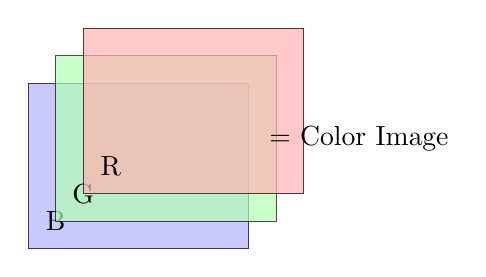
\begin{tikzpicture}[scale=0.7]
            \draw[fill=blue!30, opacity=0.7] (0,0) rectangle (4,3); \node at (0.5, 0.5) {B};
            \draw[fill=green!30, opacity=0.7] (0.5,0.5) rectangle (4.5,3.5); \node at (1, 1) {G};
            \draw[fill=red!30, opacity=0.7] (1,1) rectangle (5,4); \node at (1.5, 1.5) {R};
            \node at (6, 2) {= Color Image};
        \end{tikzpicture}
    \end{center}
    \textbf{OpenCV 的特殊性:} 默认读取顺序是 \highlight{BGR},而非 RGB。
\end{frame}

\begin{frame}{互动练习:调色盘}
    如果一个像素的 RGB 值为以下数值,它是什么颜色?
    \begin{table}
        \centering
        \begin{tabular}{cccc}
            \toprule
            R & G & B & 预测颜色 \\
            \midrule
            255 & 255 & 0 & \uncover<2->{\textcolor{yellow}{黄色}} \\
            0 & 255 & 255 & \uncover<3->{\textcolor{cyan}{青色/浅蓝}} \\
            128 & 128 & 128 & \uncover<4->{\textcolor{gray}{灰色}} \\
            0 & 0 & 0 & \uncover<5->{\textbf{黑色}} \\
            \bottomrule
        \end{tabular}
    \end{table}
\end{frame}

% -----------------------------------------------------------------------------
% 环节三:OpenCV 入门 (40分钟)
% -----------------------------------------------------------------------------
\section{OpenCV 基础}

\begin{frame}[fragile]{OpenCV 核心函数详解}
    \begin{lstlisting}[title={图像读取的隐患}]
import cv2

# 路径千万不能有中文(新手常见错误)
img = cv2.imread('paper.jpg') 

# 检查是否读取成功
if img is None:
    print("错误:文件不存在或路径含有中文!")

# 打印维度 (H, W, C)
print(img.shape) 
    \end{lstlisting}
    \begin{block}{常用 Flag}
        \begin{itemize}
            \item \texttt{cv2.IMREAD\_COLOR}:加载彩色图(默认)。
            \item \texttt{cv2.IMREAD\_GRAYSCALE}:直接以灰度模式加载(节省内存)。
        \end{itemize}
    \end{block}
\end{frame}

\begin{frame}[fragile]{Matplotlib 显示与 BGR 转换}
    为什么用 \texttt{plt.imshow} 显示出来的人脸是青蓝色的?
    \begin{lstlisting}
import matplotlib.pyplot as plt

# OpenCV 是 BGR,Matplotlib 是 RGB
img_rgb = cv2.cvtColor(img, cv2.COLOR_BGR2RGB)

plt.imshow(img_rgb)
plt.show()
    \end{lstlisting}
    \textbf{思考:} 灰度图显示时需要设置 \texttt{cmap='gray'},否则会变成“原油色”。
\end{frame}

% -----------------------------------------------------------------------------
% 环节四:图像算术运算 (30分钟)
% -----------------------------------------------------------------------------
\section{图像滤镜原理}

\begin{frame}{滤镜 1:灰度化 (Grayscale)}
    \textbf{为什么要灰度化?}
    \begin{itemize}
        \item 减少计算量(数据量降至 1/3)。
        \item 识别试卷上的文字,颜色信息通常是不必要的。
    \end{itemize}
    \textbf{原理:} $Gray = R \times 0.299 + G \times 0.587 + B \times 0.114$
    \\ (为什么绿色权重最高?因为人眼对绿色最敏感。)
\end{frame}

\begin{frame}{滤镜 2:反色 (Inversion)}
    \textbf{原理:} $NewValue = 255 - OldValue$
    \begin{itemize}
        \item 黑色 (0) $\to$ 白色 (255)
        \item 白色 (255) $\to$ 黑色 (0)
    \end{itemize}
    \textbf{应用:} 增强暗背景下的试卷特征,或者扫描负片。
\end{frame}

\begin{frame}[fragile]{滤镜 3:亮度调整与“溢出”陷阱}
    \textbf{错误做法:} \texttt{img + 50}
    \\ 如果像素值是 220,加 50 变成 270。而在 \texttt{uint8} 类型下,270 会变成 \highlight{14} (截断/绕回),导致图像出现难看的噪点。

    \begin{lstlisting}[title={安全写法}]
# 使用 numpy 的 clip 函数限制范围
bright_img = np.clip(img.astype(np.int32) + 50, 0, 255).astype(np.uint8)

# 或者使用 OpenCV 内置函数(推荐,速度更快)
bright_img = cv2.add(img, np.array([50.0]))
    \end{lstlisting}
\end{frame}

% -----------------------------------------------------------------------------
% 总结与作业
% -----------------------------------------------------------------------------
\section{总结与实战}

\begin{frame}{课堂动手环节:初探试卷图像}
    \begin{enumerate}
        \item 使用 \texttt{cv2.imread} 读取提供的 \texttt{exam.jpg}。
        \item 打印该图像的 \texttt{shape},计算总像素个数。
        \item \textbf{进阶挑战}:尝试将图像中间 $100 \times 100$ 的区域涂成纯黑色(提示:使用切片 \texttt{img[y1:y2, x1:x2] = 0})。
    \end{enumerate}
\end{frame}

\begin{frame}{课后作业:我的第一个图像处理器}
    \begin{exampleblock}{作业要求}
        编写一个 Python 脚本,读取一张照片并生成一张包含 4 张子图的对比图:
        \begin{enumerate}
            \item 原图
            \item 灰度图
            \item 亮度增强后的图
            \item 反色后的图
        \end{enumerate}
    \end{exampleblock}
    \textbf{提交方式:} 截图 + 代码。下周我们将学习如何让 AI 帮我们优化这段代码!
\end{frame}

\begin{frame}
    \begin{center}
        \Huge \textbf{Q \& A}
        \vspace{1cm}
        \Large 准备好进入计算机视觉的世界了吗?
    \end{center}
\end{frame}

\end{document}